\documentclass{article}

\usepackage{fullpage}
\usepackage{amsmath,amssymb}
\usepackage{cleveref}
\usepackage{graphicx}

\newcommand{\NB}{\mbox{NB}}
\newcommand{\lik}{\mathcal{L}}
\newcommand{\var}{\mbox{var}}
\newcommand{\ep}{\varepsilon}

\begin{document}

\section{Background}

Count data describe the number of times an event occurs and take on non-negative integer values. These data cannot be described by continuous distributions, such as the normal distribution; instead, discrete distributions must be used. This section describes various discrete distributions that can be used to build a count data version of the stochastic frontier model. First, unbounded distributions like the Poisson and negative binomial distributions are described and applications to generalized linear models are explored. Then, bounded distributions that can be used to model one-sided errors, such as the binomial and beta-binomial distributions, are detailed.

As a matter of notation, let $y$ be a $N\times 1$ vector of count outcome data, $X$ be a $N\times k$ matrix of explanatory variables, and let $\beta$ be a $k\times 1$ vector of slope parameters, where $N$ is the number of observations in the data and $k$ is the number of explanatory variables. Further, let $\lik$ denote the likelihood function, and let $i$ subscripts denote the $i$th observation/row of a variable.

\subsection{Traditional Stochastic Frontier Models}

A typical stochastic frontier model has the form
\begin{equation}
y_i = X_i\beta - \delta_i + \ep_i,
\end{equation}
where $\ep_i$ is a two-sided measurement error and $\delta_i$ is a one-sided error representing inefficiency. We will make common assumptions that $\ep_i\sim N(0, \sigma_\ep^2)$ and $\delta_i\sim N^+(\mu_\delta, \sigma_\delta^2)$. Two methods can be employed to compute the likelihood. First, the law of total probability can be used to integrate directly over $\delta$:
\begin{equation}
	f(y_i | \beta, \sigma_\ep, \mu_\delta, \sigma_\delta) = \int_{\delta_i} f(y_i | \beta, \sigma_\ep, \delta_i) f(\delta_i | \mu_\delta, \sigma_\delta) d\delta_i.
\end{equation}
Note that this integral must be evaluated for each observation and therefore does not scale well. Alternatively, it can be shown that
\begin{equation}
	
\end{equation}

\subsection{Poisson and Negative Binomial Count Models}

The Poisson distribution is commonly used to model count data outcomes. The Poisson distribution is characterized by the likelihood
\begin{equation}
	\lik(y_i | \lambda) = \frac{\lambda^{y_i}e^{-\lambda}}{y_i!},
\end{equation}
where $\lambda>0$ is a parameter. The outcome $y_i$ can take on any non-negative integer value, and the Poisson distribution is therefore unbounded. A key feature of the Poisson distribution is that $E[y_i] = \var(y_i) = \lambda$, leading to two consequences. First, a generalized linear model can be constructed by setting $\lambda = \exp(X_i\beta)$, and therefore $E[y_i] = \exp(X_i\beta)$. Second, since a single parameter controls both mean and variance, data can be over-dispersed (common) or under-dispersed (less common) relative to the model with no method of correction.

The negative binomial distribution provides one method of correcting for over-dispersion relative to the Poisson distribution. There are several parameterizations of the negative binomial distribution; in this document we will use the likelihood of the form
\begin{equation}
	\lik(y_i | \mu, \phi) = {{y_i + \phi - 1}\choose{y_i}} \left(\frac{\mu}{\mu + \phi}\right)^{y_i} \left(\frac{\phi}{\mu + \phi}\right)^\phi,
\end{equation}
where $\mu>0$ and $\phi>0$ are parameters of the distribution. Under this formulation, $E[y_i] = \mu$ and $\var(y_i) = \mu + \mu^2 / \phi$. Notice that $\var(y_i) > \mu$, thereby accommodating data with higher variance than the Poisson distribution. As with the Poisson distribution, the negative binomial distribution can be made into a generalized linear model by setting $\mu = \exp(X_i\beta)$. The parameters $\beta$ and $\phi$ are then free to be estimated.

\begin{figure}
	\centering
	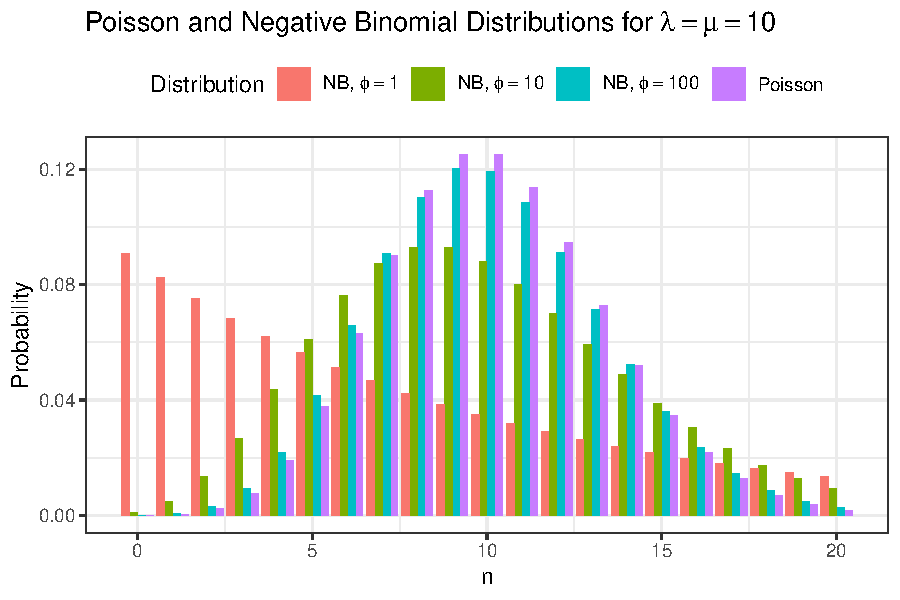
\includegraphics[width=6in]{plotting/poisson-nb.pdf}
	\caption{Comparison of Poisson and Negative Binomial Distributions}
	\label{fig:poisson-nb}
\end{figure}

A comparison of Poisson and negative binomial mass functions is shown in \cref{fig:poisson-nb}. Each of the distributions shown has the same mean, and the $\phi$ parameter is adjusted in the negative binomial distribution to increase variance.

\end{document}
